%                                                                 aa.dem
% AA vers. 9.1, LaTeX class for Astronomy & Astrophysics
% demonstration file
%                                                       (c) EDP Sciences
%-----------------------------------------------------------------------
%
%\documentclass[referee]{aa} % for a referee version
%\documentclass[onecolumn]{aa} % for a paper on 1 column  
%\documentclass[longauth]{aa} % for the long lists of affiliations 
%\documentclass[letter]{aa} % for the letters 
%\documentclass[bibyear]{aa} % if the references are not structured 
%                              according to the author-year natbib style

%
% \documentclass[draft]{aa} 
\documentclass{aa}

%
\usepackage{graphicx}
%%%%%%%%%%%%%%%%%%%%%%%%%%%%%%%%%%%%%%%%
\usepackage{txfonts}
%%%%%%%%%%%%%%%%%%%%%%%%%%%%%%%%%%%%%%%%
%\usepackage[options]{hyperref}
% To add links in your PDF file, use the package "hyperref"
% with options according to your LaTeX or PDFLaTeX drivers.
%
\usepackage[]{hyperref}
\hypersetup{colorlinks=true, urlcolor=blue, citecolor=cyan, pdfborder={0 0 0}}

\begin{document} 


\title{An analysis of the most distant catalogued open clusters}
\subtitle{Re-assessing fundamental parameters with Gaia EDR3 and \texttt{ASteCA}}

\author{G. I. Perren\inst{1}
      \and
      M. S. Pera\inst{1}
      \and
      H. Navone\inst{2}
      \and
      R. A. Vázquez\inst{1,3}
      % \fnmsep\thanks{Just to show the usage
      % of the elements in the author field}
}

\institute{Instituto de Astrof\'isica de La Plata (IALP-CONICET), La Plata,
Argentina\\
\email{gabrielperren@gmail.com}
\and
Facultad de Ciencias Exactas, Ingeniería y Agrimensura (UNR-IFIR-CONICET),
Rosario, Argentina
\and
Facultad de Ciencias Astronómicas y Geofísicas (UNLP-IALP-CONICET), 1900 La
Plata, Argentina
% \thanks{The university of heaven temporarily does not
%         accept e-mails}
}
\date{Received September 15, 2021; accepted December 16, 2021}

% \abstract{}{}{}{}{} 
% 5 {} token are mandatory
 
\abstract
% context heading (optional)
% {} leave it empty if necessary  
{Several studies have been presented in the last few years applying some kind of
automatic processing of data to estimate the fundamental parameters of open
clusters. These parameters are later on employed in larger scale analyses, for
example the structure of the Galaxy's spiral arms.
The distance is one of the more straightforward parameters to estimate, yet
enormous differences can still be found among published data. This is
particularly true for open clusters located more than a few Kpc away.}
% aims heading (mandatory)
{
We cross-matched several published catalogues and selected the twenty-five most
distant open clusters ($>$9000 Kpc). We then performed a detailed analysis of
their fundamental parameters, with emphasis on their distances, to determine the
agreement between catalogues and our estimates.}
% methods heading (mandatory)
{Photometric and astrometric data from the Gaia EDR3 survey was employed. The
data was processed with our own membership analysis code (pyUPMASK), and our
package for automatic fundamental cluster's parameters estimation
(\texttt{ASteCA}).}
% results heading (mandatory)
{We find differences in the estimated distances of up to several Kpc
between our results and those catalogued, even for the catalogues that show the
best matches with \texttt{ASteCA} values. Large differences are also found for
the age estimates.}
% conclusions heading (optional), leave it empty if necessary 
{Caution is thus strongly recommended when using catalogued parameters of open
clusters to infer large-scale properties of the Galaxy, particularly for those
located more than a few Kpc away.}

\keywords{
  Methods: statistical --
  Galaxies: star clusters: general --
  (Galaxy:) open clusters and associations: general --
  Techniques: photometric--
  Parallaxes --
  Proper motions
}

\maketitle


\section{Introduction}

 The unprecedented amount of high precision data for parallaxes and photometry provided by the Gaia mission in successive deliveries (GDR2 and EGDR3, \cite{Gaia_2016,Gaia_EDR3}) offers us a unique opportunity to get the fundamental parameters, age, distance, the observed mass and the metal content of open clusters, OC. Indeed, the arrival of new techniques for analyzing massive data 
 combined with the increasing data precision promise more reliable results than those obtained with the old techniques mostly based on the visual inspection of their color-magnitude diagrams and isochrone fittings \citep{Phelps1994} or on direct comparison with HR diagrams of synthetic clusters \citep{Siess1997}. Automated processes such as the one applied by \cite{Kharchenko_2012} have also played an important role in determining cluster parameters in a massive way. But the continuous increasing of high quality data is a defying circumstance where a variety of analysis are being considered even including artificial neural networks \citep{Cantat_2020} combined with new strategies for determining cluster memberships \citep{Krone2014,Cantat2018}. The intrinsic value of studying OCs has been profusely described in several opportunities and we are not going to repeat them here. However a brief enumeration of the importance of these object is appropriate: the oldest OCs allow us to investigate the extension in height and radial extension of the galactic disk; old OCs tell us about the chemical history, the mixing processes and the processes of OCs destruction by interaction with other populations of the galaxy as well as the age-metallicity relationship \citep{Friel1995,Tosi2004,Hayes2015}. The youngest OCs, on the other hand, are not only used as laboratories to investigate stellar evolution (they allow studying in detail the boundary conditions necessary to create new generations of stars (\citep{Lada2003}) but are also routinely employed too in the analysis of the Milky Way's structure~\citep{Loktin_1992,Moitinho_2006,Vazquez2008,Moitinho_2010} becoming particularly
 useful in the tracing of spiral arms~\citep{carraro_2013,Molina_2018}. It is unfortunate that young OCs are mainly arranged along the 
galactic disk where the strong visual absorption and the contamination by 
field stars very often prevent observing stars in the lower part of the sequence of 
these objects. In this sense, the situation is not much better at all for the older OCs. In fact, these objects do not have very luminous stars in the main sequence, although they do in the giant branch. Notwithstanding, stars in the lower part of their sequences as well as those ones belonging to the giant branch share similar photometric characteristics with field stars making difficult to unravel which population each star belongs to (\cite{Hayes2015}). 
The situation worsens as the distance to the older OCs increases because the limiting magnitude is increasing and if this happens only a small portion 
of the lower part is usually divisible. But it is not only the photometric space that is disturbed by distance. The proper motions of far OCs are difficult to separate clearly from those characterizing the field population against which we see them projected, therefore introducing an additional degree of confusion in determining memberships.

Our interest in this current article is twofold. On the one hand, it is focused on reexamining the distances
and properties of the most distant OCs cataloged so far in our galaxy, say 
those at more than 9 kpc from the sun. A total of 25 clusters were found by inspection 
in four different recognized databases that satisfy this requirement as we will 
explain below. However, these bases show great differences in the parameters 
determined for them, both in distances and in ages. In part the differences in the 
parameters of the same object may be due to the different techniques used to obtain 
them combined with the problem of the enormous distance at which they are. However, 
it is of great interest that most of them included in recent catalogs made with advanced 
analysis techniques are indicated to be clusters older than one billion years. 
But in some other catalogs these same clusters have relatively small ages and shorter 
distances as well. We certainly want to contribute with our analysis to resolve the 
origin of these differences.
On a side, we want to compare our new membership estimation technique, as explained below, in combination with ASteCA, et ....


 This article is structured as follows. In Sect~\ref{sec:cat_clust_data} we
 introduce the stellar cluster catalogues, the clusters selected to be
 analyzed (crossed-matched from those catalogues), and the photometric and 
 astrometric data used to perform the analysis. Sect~\ref{sec:clust_analy}
 presents the methods employed in the study of all the clusters. The comparison
 of the estimated parameters with the catalogued values for each cluster is done
 in Sect~\ref{sec:results}. Finally, conclusions are highlighted in
 Sect~\ref{sec:conclusions}.





% =============================================================================
\section{Catalogues, clusters, and data}
 \label{sec:cat_clust_data}

 We chose four catalogues to cross-match and subsequently select the most
 distant clusters: \citet[][New Catalog of Optically Visible Open Clusters and
 Candidates, hereinafter OC]{Dias_2002},~\citet[][WEBDA,\footnote{
 \url{https://webda.physics.muni.cz/}} hereinafter WB]{Netopil_2012},
 \citet[][Milky Way Star Clusters Catalog, hereinafter MW]{Kharchenko_2012},
 and~\citet[][hereinafter CG]{Cantat_2020}.
 %
 The first two (OC and WB) are compilations of open clusters' fundamental
 parameters from the literature. They contain around 1700 (WB) and 2100 
 (OC) entries, and are heavily used in the field of open cluster research.
 The parameter values in both catalogues are heterogeneous, being compiled from
 various sources.
 The MW catalog is the largest one ($\sim$3000 entries) and, similarly to the CG
 catalog ($\sim$2000 entries), is composed of homogeneous fundamental parameter
 values obtained for all its entries. The method employed by the authors of the
 MW catalog is a semi-automated isochrone fit, while the CG catalog was
 generated employing an artificial neural network (trained on parameter values
 taken from the literature).

 Since we are interested in the open clusters most distant from the Sun, we
 select from these cross-matched catalogues those that are located at a
 distance of 9 Kpc or more in either of them. This is an arbitrary value that
 results in enough clusters to draw general conclusions, but not too many that
 would impede their detailed analysis.
 The initial full list consisted of thirty-eight open clusters. Eleven of these
 were found only in the MW catalog with distances larger than 9000 pc. These are
 either listed with substantially smaller distances in the other catalogs, or
 too sparse and or dubious. Hence these clusters were removed from the
 cross-matched list.
 %
 Two other clusters were also removed: Shorlin 1 ($\alpha_{2000}$=166.44,
 $\delta_{2000}$=-61.23) and FSR0338
 ($\alpha_{2000}$=327.93, $\delta_{2000}$=55.33). The latter appears in WB and
 MW at a distance of 12600 pc and 5600 pc respectively, while the former is
 listed only in MW with a distance of 14655 pc. Shorlin1 is studied
 in~\cite{Carraro_2009} and~\cite{Turner_2012}; in both cases the authors
 conclude that this is not a real cluster but a grouping of young stars.
 % Shorlin 1
 %
 % Carraro & Costa (2009)
 % > We also present evidence that this extremely distant group, formerly assumed
 % to be a star cluster (Shorlin 1), is a diffuse, young population, typically
 % found in spiral galaxies.
 %
 % Turner (2012)
 % > ...star counts also imply that Shorlin 1 is unlikely to represent a true
 % cluster, but is instead merely the trapezium-like remains of a previously-
 % bound cluster with an implied age of only a few Myr, according to the likely
 % presence of O-type stars within its boundaries.
 %
 FSR0338 is analyzed in~\cite{Froebrich_2010} where a distance of 6000 pc is
 assigned, but with large uncertainties.
 % Froebrich et al. (2010)
 % > Th high probability members of this newly identified cluster seem to indicate
 % an object with an age of 0.4 Gyrs at a distance of 6 kpc. The scatter in the
 % data points suggests larger than normal uncertainties for the parameters.
 %
 In both cases we find no evidence of a true stellar cluster in these regions.
 We base our conclusion on two findings. First, the large proper motions
 dispersion of the stars that occupy the overdensity around the central
 coordinates assigned to either object. Second, the lack of a clear sequence in
 their respective color-magnitude diagrams (CMD). These two clusters are thus
 discarded from further analysis. The remaining twenty-five clusters that will
 be studied in this work are shown in Table~\ref{tab:clusters}. Most of the
 selected clusters are located in the Third Quadrant with all of them in the
 latitude range of [-12$^{\circ}$, 8$^{\circ}$], relatively close to the
 galactic plane.

 \begin{table*}
 \caption{Selected catalogued open clusters with a distance $\geq$9000 pc,
 ordered by right ascension. The ages are expressed as the logarithm, and the
 distances are in parsec. In parenthesis, the short names used for the clusters
 throughout the article. Clusters with no distances below the 9000 pc limit in
 any of the catalogs are marked with boldface.}
 \label{tab:clusters}
 \centering
 % \begin{tabular}{lcccccccccc}
 \begin{tabular}{lllllllllll}
 \hline\hline
 Cluster & $\alpha_{2000}$  & $\delta_{2000}$ & OC$_{age}$ & OC$_{dist}$ & CG$_{age}$ &
 CG$_{dist}$ & WB$_{age}$ & WB$_{dist}$ & MW$_{age}$ & MW$_{dist}$ \\
 \hline
 Berkeley 73 (BER73)     & 95.5   & -6.35     & 9.18  & 9800  & 9.15  & 6158  &
 9.36 & 6850 & 9.15  & 7881  \\
 Berkeley 25 (BER25)     & 100.25 & -16.52    & 9.7   & 11400 & 9.39  & 6780  &
 9.6   & 11300 &  9.7   & 11400 \\
 Berkeley  75 (BER75)     & 102.25 & -24       & 9.6   & 9100  & 9.23  &  8304 
 & 9.48  & 9800  & 9.3   & 6273  \\
 Berkeley  26 (BER26)     & 102.58 & 5.75      & 9.6   & 12589 & -   & -   & 9.6
 & 4300  & 8.71  & 2724  \\
 Berkeley  29 (\textbf{BER29})     & 103.27 & 16.93     & 9.025 & 14871 & 9.49  & 12604 &
 9.025 & 14871 & 9.1   & 10797 \\
 Tombaugh 2 (TOMB2)     & 105.77 & -20.82    & 9.01  & 6080  & 9.21  & 9316  &
 9.01 & 13260 & 9.01  & 6565  \\
 Berkeley 76 (BER76)     & 106.67 & -11.73    & 9.18  & 12600 & 9.22  & 4746  &
 9.18 & 12600 & 8.87  & 2360  \\
 FSR 1212 (F1212)   & 106.94 & -14.15    & -   & -   & 9.14  & 9682  & -   & -
 & 8.65  & 1780  \\
 Saurer 1 (\textbf{SAU1})   & 110.23 & 1.81      & 9.7   & 13200 & -   & -   & 9.85  &
 13200 & 9.6   & 13719 \\
 Czernik 30 (CZER30)    & 112.83 & -9.97     & 9.4   & 9120  & 9.46  & 6647  &
 9.4 & 6200  & 9.2   & 6812  \\
 Arp-Madore 2 (\textbf{ARPM2})     & 114.69 & -33.84    & 9.335 & 13341 & 9.48  & 11751 &
 9.335 & 13341 & 9.335 & 13338 \\
 vd Bergh-Hagen 4 (\textbf{BH4})     & 114.43 & -36.07    & -   & -   & -   & -  
 & 8.3   & 19300 & -   & -   \\
 FSR 1419 (F1419)   & 124.71 & -47.79    & -   & -   & 9.21  & 11165 & -   & -   & 8.375 & 7746  \\
 vd Bergh-Hagen 37 (BH37)    & 128.95 & -43.62    & 8.84  & 11220 & 8.24 
 & 4038  & 8.85  & 2500  & 7.5   & 5202  \\
 ESO 092 05 (E9205)  & 150.81 & -64.75    & 9.3   & 5168  & 9.65  & 12444 &
 9.78  & 10900 & 9.3   & 5168  \\
 ESO 092 18 (E9218)  & 153.74 & -64.61    & 9.024 & 10607 & 9.46  & 9910  &
 9.024 & 607   & 9.15  & 9548  \\
 Saurer 3 (SAU3)   & 160.35 & -55.31    & 9.3   & 9550  & -   & -   & 9.45  &
 8830 & 9.3   & 7075  \\
 Kronberger 39 (KRON39)    & 163.56 & -61.74    & -   & 11100 & -   & -   & -   &
 -   & 6     & 4372  \\
 ESO 093 08 (E9308)  & 169.92 & -65.22    & 9.74  & 14000 & -   & -   & 9.65  &
 3700  & 9.8   & 13797 \\
 vd Bergh-Hagen 144 (BH144)   & 198.78 & -65.92    & 8.9   & 12000 & 9.17
 & 9649  & 8.9   & 12000 & 9     & 7241  \\
 vd Bergh-Hagen 176 (BH176)   & 234.85 & -50.05    & -   & -   & -   & - 
 & -   & 13400 & 9.8   & 18887 \\
 Kronberger 31 (\textbf{KRON31})    & 295.05 & 26.26     & -   & 11900 & -   & -   & -   &
 -   & 8.5   & 12617 \\
 Saurer 6 (SAU6)   & 297.76 & 32.24     & 9.29  & 9330  & -   & -   & 9.29  &
 9330 & 9.2   & 7329  \\
 Berkeley 56 (\textbf{BER56})     & 319.43 & 41.83     & 9.6   & 12100 & 9.47  & 9516  &
 9.6 & 12100 & 9.4   & 13180 \\
 Berkeley 102 (BER102)    & 354.66 & 56.64     & 9.5   & 9638  & 9.59  & 10519 &
 8.78  & 2600  & 9.14  & 4900 \\
 \hline
 \end{tabular}
 \end{table*}

 There are two other major works where a large catalog of analyzed open clusters
 is presented: \cite{Lui_2019} and \cite{Dias_2021}. The latter does not contain
 clusters with such large distances, and was hence not used. The former lists
 only four, and their values will be included in the discussion of the results
 in Sect.~\ref{sec:results}.\\

 Data from Gaia EDR3~\citep{Gaia_2016,Gaia_EDR3} was retrieved for a box of 20
 arcmin of length around the central coordinates for all the clusters.

 % A small synopsis for each cluster is presented below, in alphabetical order:\\
 % \noindent\textbf{Kronberger31} and \textbf{Kronberger39}: these two clusters
 % where discovered and catalogued as \emph{Cluster candidates with RCs}
 % in~\cite{Kronberger_2006}. Both show a very dispersed and scarcely populated
 % sequence.\\



 In Fig~\ref{fig:MWmap} we show the twenty-five selected clusters for each of
 the four catalogues, positioned on the face-on view of the Galaxy The spiral
 arms are taken from~\cite{Momany_2006}. The large dispersion for the distances
 assigned to each cluster in different catalogs is clearly visible.

 \begin{figure*}
  \resizebox{\hsize}{!}{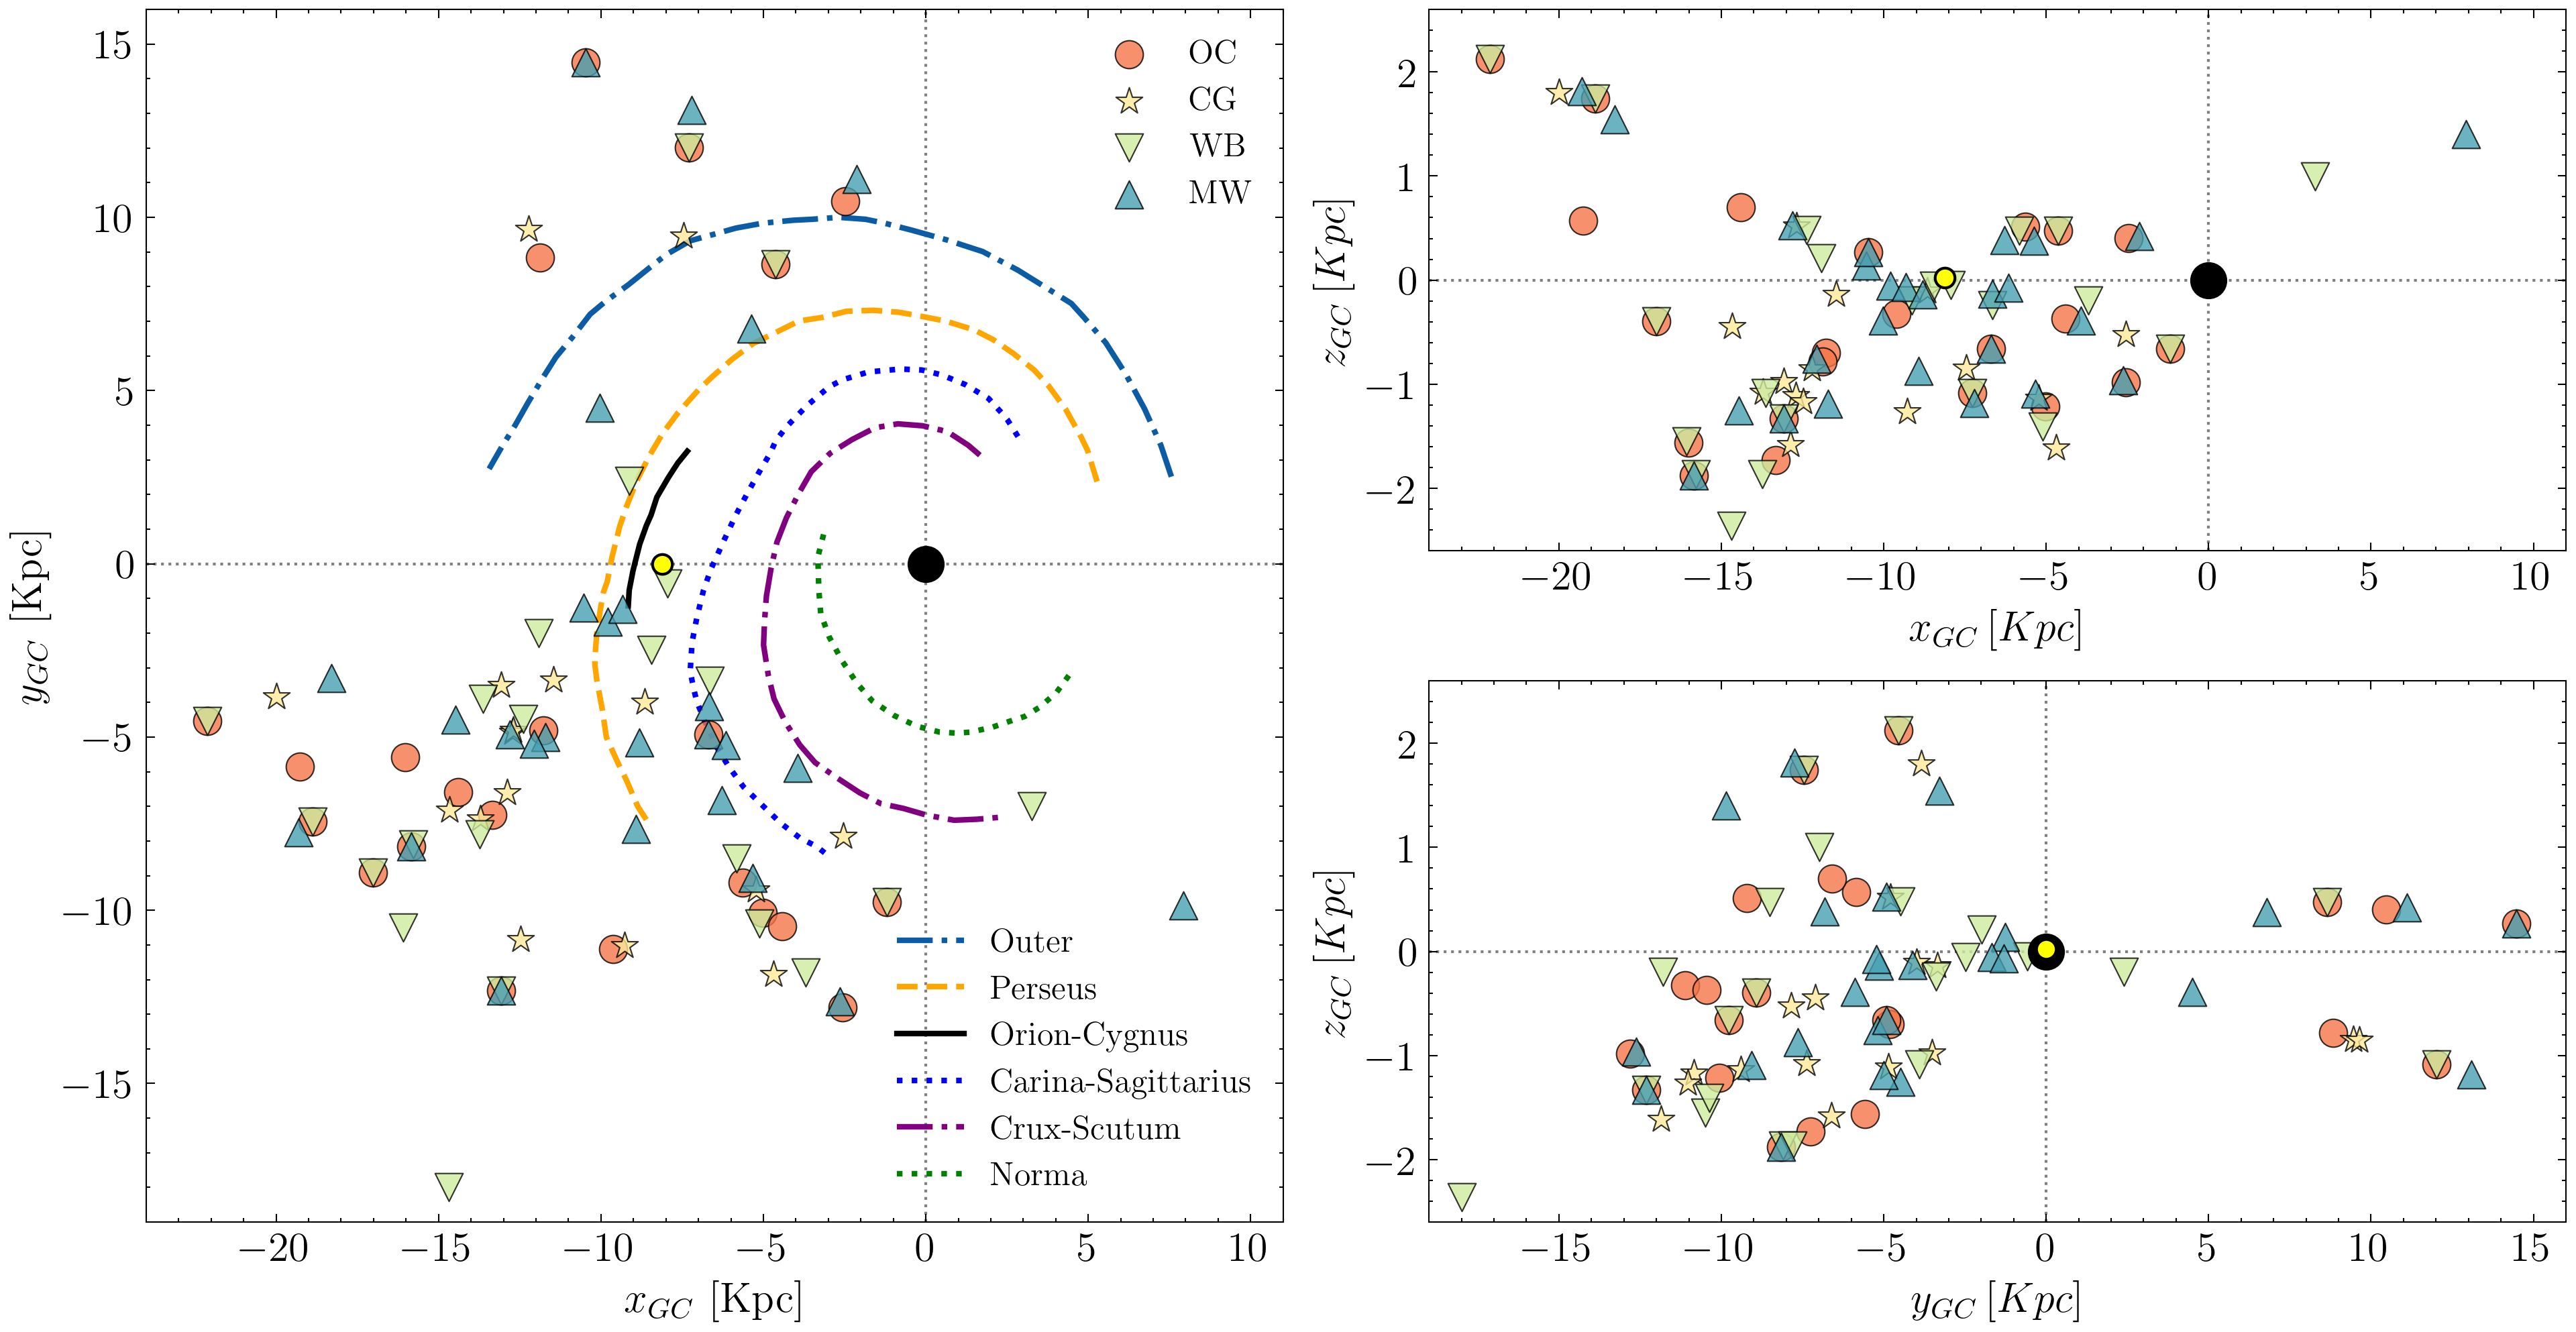
\includegraphics[]{figs/MWmap.png}}
  \caption{Top: position of the twenty-five clusters selected from the four
  catalogs mentioned in the text, on a face-on view of the Milky Way. The Sun
  and the center of the Galaxy are marked with a yellow filled circle and a
  black filled circle, respectively. Bottom: edge-on views, same color and
  marker conventions as above.}
  \label{fig:MWmap}
 \end{figure*}





% =============================================================================
\section{Cluster analysis}
 \label{sec:clust_analy}

 The first step in the cluster analysis is the estimation of their structural
 properties, i.e. center coordinates and limiting radius. Although centers and
 diameters are present in (some of) the catalogues, not all of these values are
 correct. We use our \texttt{ASteCA} package
 \citep{Perren_2015}\footnote{\url{http://asteca.github.io/}} throughout this
 work to perform the structural and fundamental parameters analysis. We have
 applied this tool to the study of hundreds of clusters in previous articles,
 with excellent results~\citep{Perren_2017,Perren_2020}.

 The center values are obtained after applying a two-dimensional kernel density
 analysis (KDE) on each of the cluster's coordinates. This method assigns the
 center of the cluster to the point with the largest density in the frame. 

  \begin{table}
  \caption{xxx}
  \label{tab:radii}
  \centering
  \begin{tabular}{llll}
  \hline\hline
  Cluster & $r_{c}$  &  $r_{t}$ & radius\\
  \hline
   BER73         & 0.6$_{0.5}^{0.7}$ &  4.9$_{3.8}^{6.3}$ &  2.0\\
   BER25         & 1.5$_{1.2}^{1.8}$ &  7.0$_{6.2}^{8.0}$ &  5.0\\
   BER75         & 0.4$_{0.3}^{0.5}$ &  5.0$_{3.6}^{6.6}$ &  2.0\\
   BER26         & 0.7$_{0.5}^{1.0}$ &  3.4$_{2.5}^{4.5}$ &  1.6\\
   BER29         & 0.5$_{0.4}^{0.5}$ &  7.4$_{6.4}^{8.6}$ &  3.0\\
   TOMB2         & 0.9$_{0.8}^{0.9}$ &  6.7$_{6.1}^{7.4}$ &  3.5\\
   BER76         & 1.6$_{1.2}^{2.5}$ &  7.4$_{5.7}^{9.6}$ &  4.0\\
   F1212         & 0.8$_{0.6}^{1.1}$ &  8.8$_{6.6}^{10.7}$ & 3.0\\
   SAU1          & 0.7$_{0.5}^{1.0}$ &  3.9$_{2.9}^{5.4}$ &  2.0\\
   CZER30        & 0.6$_{0.4}^{0.7}$ &  6.4$_{4.8}^{8.2}$ &  2.5\\
   ARPM2         & 1.4$_{1.0}^{2.0}$ &  4.1$_{3.4}^{4.9}$ &  3.0\\
   BH4           & 0.4$_{0.3}^{0.5}$ &  5.7$_{4.0}^{7.1}$ &  2.0\\
   F1419         & 1.2$_{0.9}^{1.8}$ &  6.0$_{4.3}^{8.3}$ &  3.0\\
   BH37          & 1.2$_{0.8}^{1.9}$ &  3.8$_{2.5}^{5.6}$ &  2.0\\
   E9205         & 1.0$_{0.9}^{1.3}$ &  4.4$_{3.7}^{5.3}$ &  3.0\\
   E9218         & 0.6$_{0.6}^{0.7}$ &  6.5$_{5.9}^{7.3}$ &  3.0\\
   SAU3          & 0.5$_{0.4}^{0.6}$ &  4.9$_{3.8}^{6.4}$ &  2.0\\
   KRON39        & 0.3$_{0.2}^{0.3}$ &  5.6$_{4.1}^{7.0}$ &  2.0\\
   E9308         & 0.2$_{0.2}^{0.2}$ &  5.0$_{4.2}^{5.7}$ &  1.5\\
   BH144         & 0.3$_{0.3}^{0.4}$ &  2.8$_{2.3}^{3.4}$ &  1.5\\
   BH176         & 0.6$_{0.5}^{0.7}$ &  4.6$_{3.8}^{5.8}$ &  2.0\\
   KRON31        & 0.5$_{0.4}^{0.6}$ &  6.9$_{5.7}^{7.6}$ &  2.0\\
   SAU6          & 0.5$_{0.4}^{0.7}$ &  3.7$_{2.9}^{4.8}$ &  2.0\\
   BER56         & 1.6$_{1.4}^{1.7}$ &  8.1$_{7.4}^{8.9}$ &  4.5\\
   BER102        & 1.0$_{0.8}^{1.5}$ &  3.8$_{3.0}^{4.9}$ &  2.5\\
  \hline
  \end{tabular}
  \end{table}


 \begin{figure*}
  \resizebox{\hsize}{!}{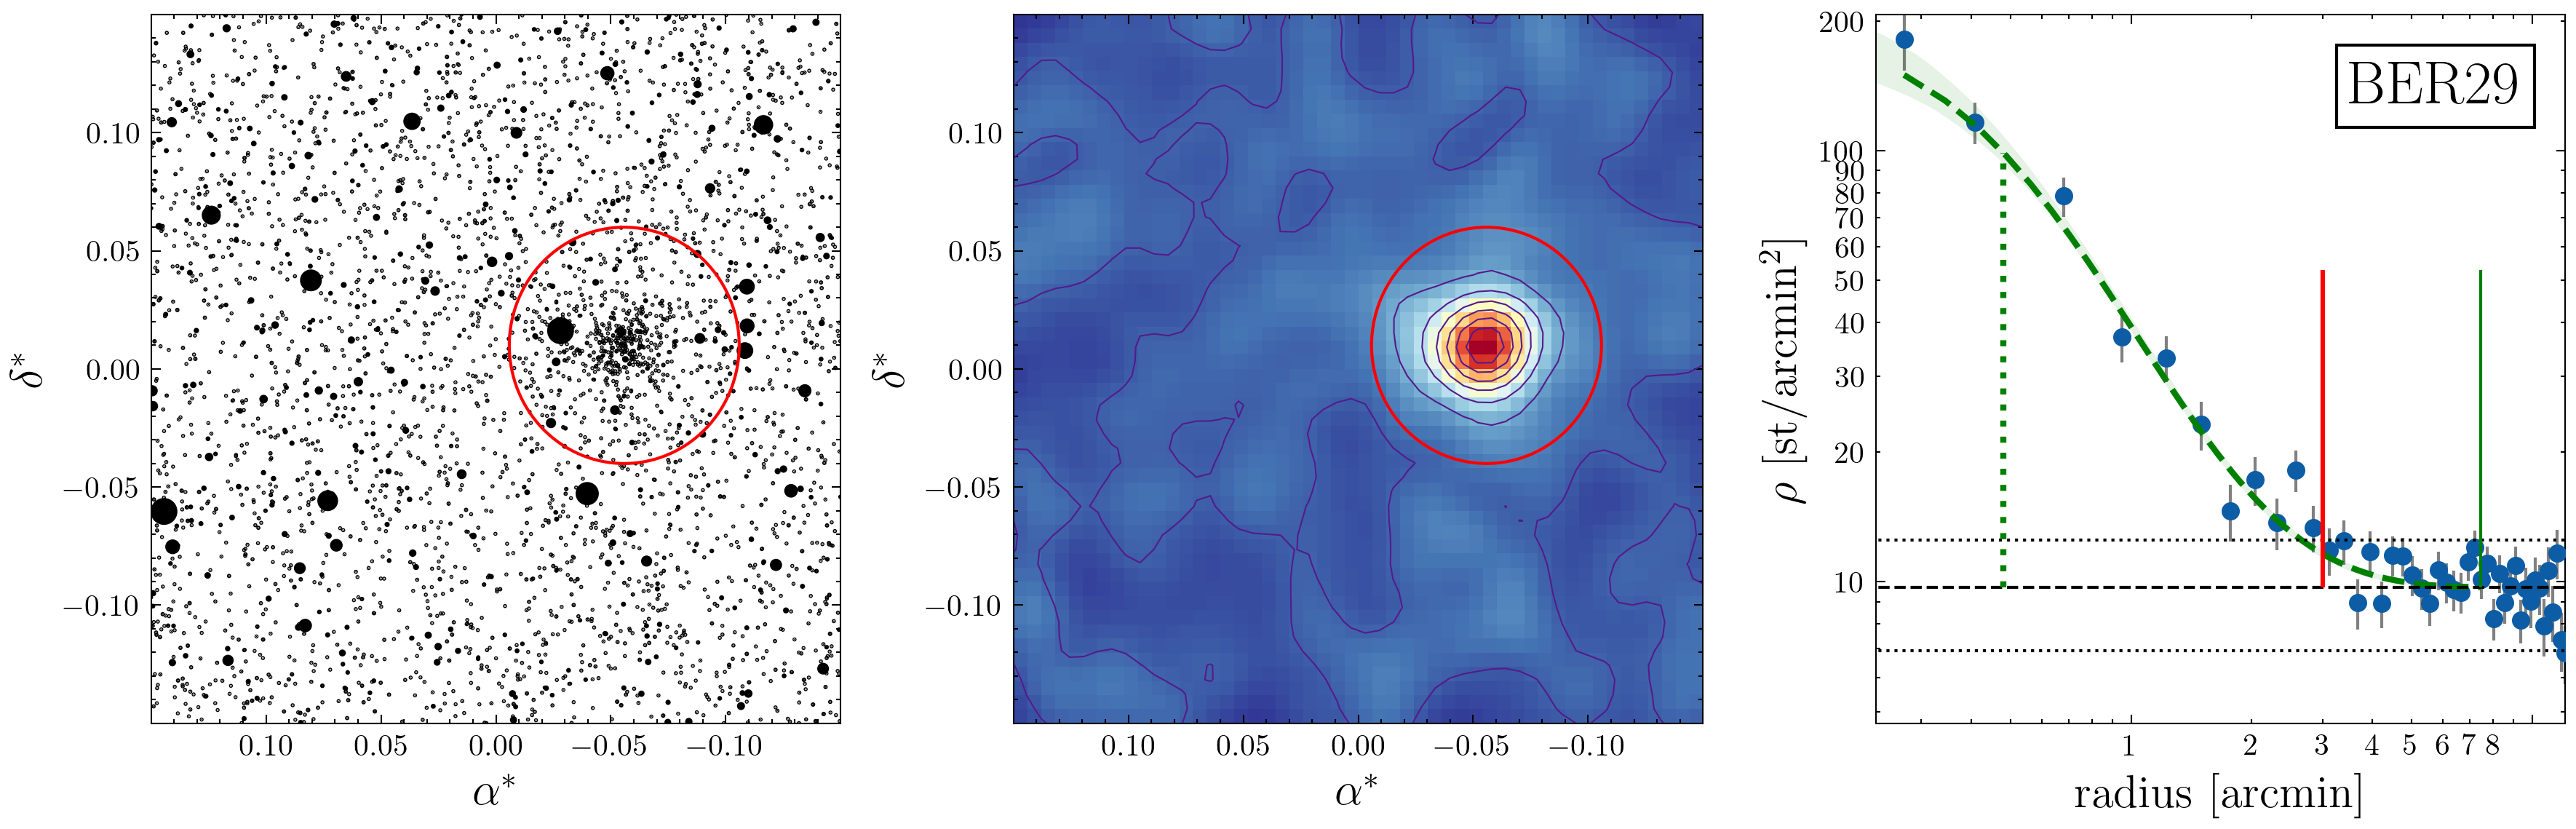
\includegraphics[]{figs/BER29_struct.png}}
  \caption{xxx}
  \label{fig:BER29_struct}
 \end{figure*}


 \begin{figure*}
  \resizebox{\hsize}{!}{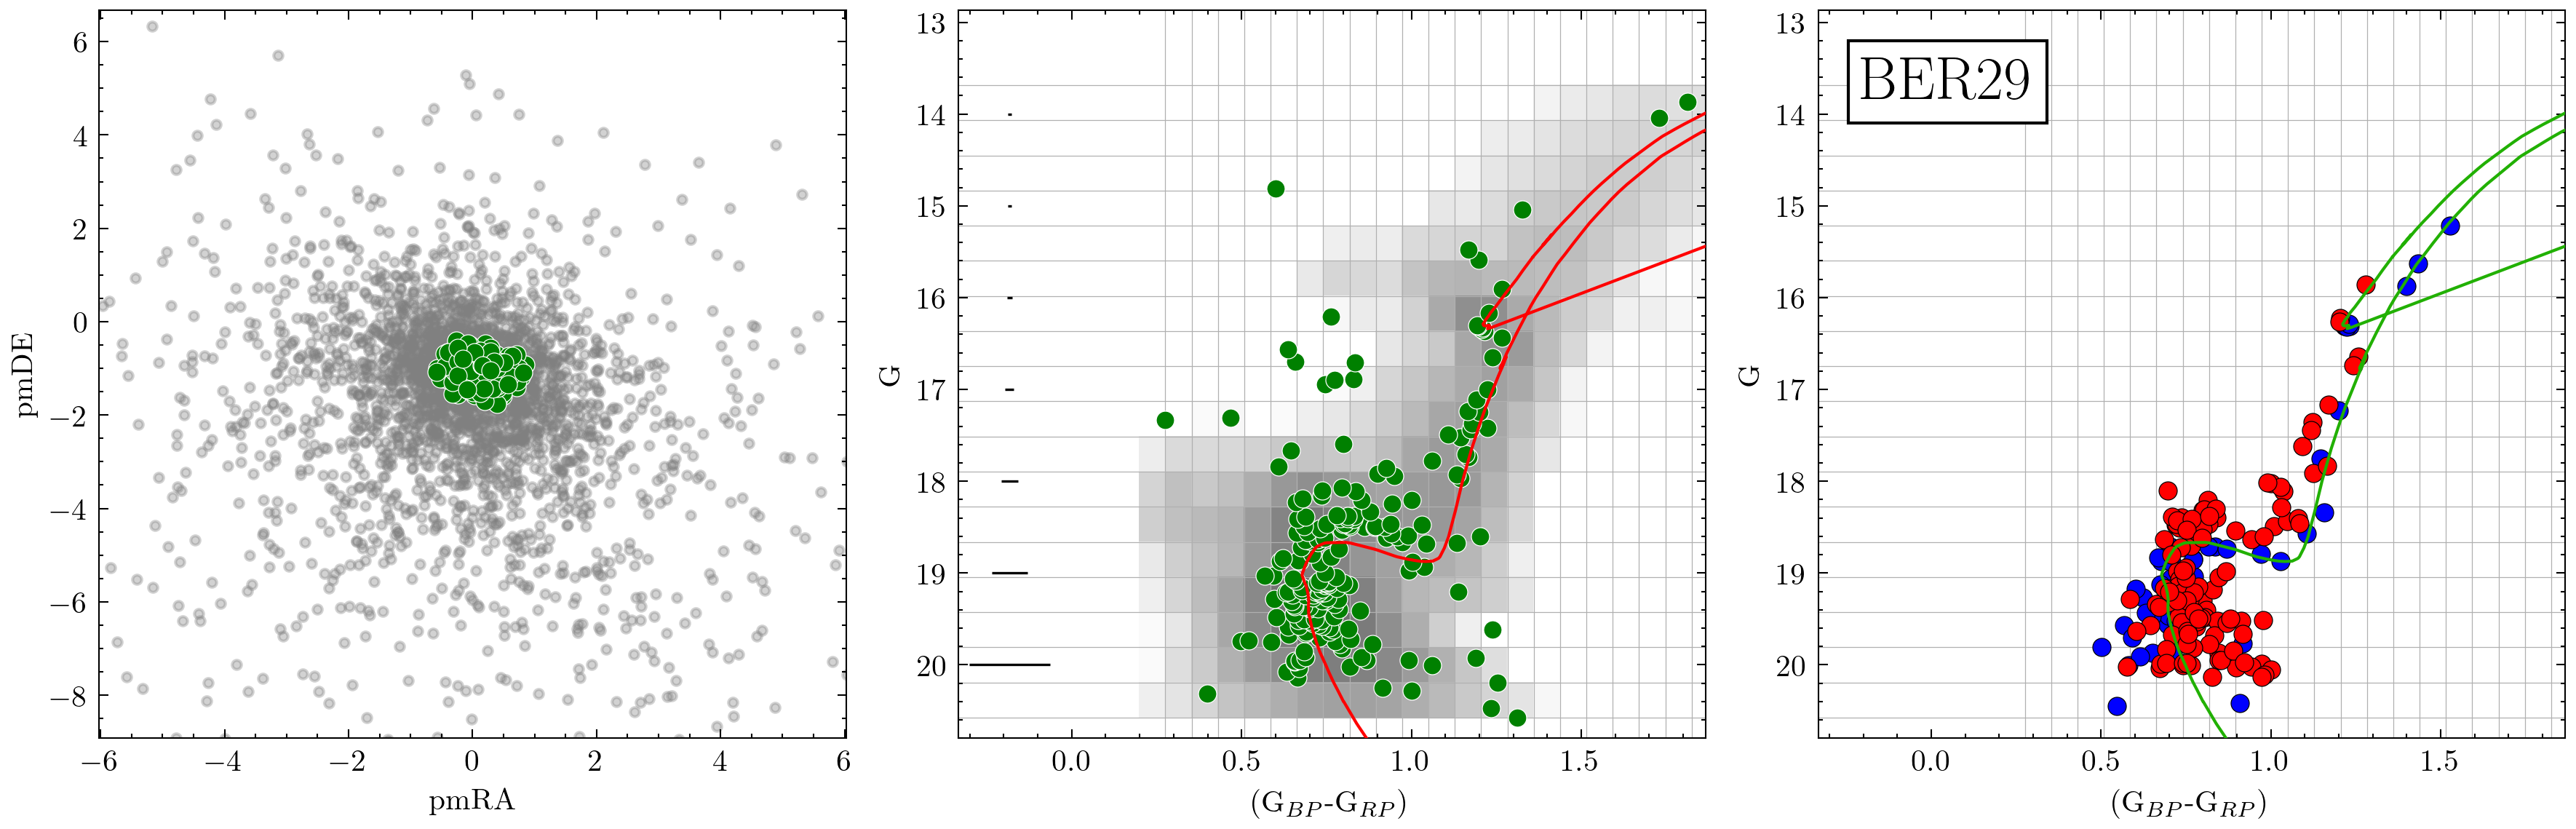
\includegraphics[]{figs/BER29_fpars.png}}
  \caption{xxx}
  \label{fig:BER29_fpars}
 \end{figure*}





% =============================================================================
\section{Results}
 \label{sec:results}

 xxxxx





% =============================================================================
\section{Conclusions}
 \label{sec:conclusions}

 xxxxx




   %--------------------------------------------------- One column table
%    \begin{table}
%       \caption[]{Opacity sources.}
%          \label{KapSou}
%      $$ 
%          \begin{array}{p{0.5\linewidth}l}
%             \hline
%             \noalign{\smallskip}
%             Source      &  T / {[\mathrm{K}]} \\
%             \noalign{\smallskip}
%             \hline
%             \noalign{\smallskip}
%             Yorke 1979, Yorke 1980a & \leq 1700^{\mathrm{a}}     \\
% %           Yorke 1979, Yorke 1980a & \leq 1700             \\
%             Kr\"ugel 1971           & 1700 \leq T \leq 5000 \\
%             Cox \& Stewart 1969     & 5000 \leq             \\
%             \noalign{\smallskip}
%             \hline
%          \end{array}
%      $$ 
%    \end{table}



%                                                One column figure
%----------------------------------------------------------------- 
% \begin{figure}
% \centering
% %%%\includegraphics[width=3cm]{empty.eps}
%    \caption{Vibrational stability equation of state
%             $S_{\mathrm{vib}}(\lg e, \lg \rho)$.
%             $>0$ means vibrational stability.
%            }
%       \label{FigVibStab}
% \end{figure}

\section{Conclusions}

xxx

\begin{acknowledgements}
This work has made use of data from the European Space Agency (ESA) mission
{\it Gaia} (\url{https://www.cosmos.esa.int/gaia}), processed by the {\it Gaia}
Data Processing and Analysis Consortium (DPAC,
\url{https://www.cosmos.esa.int/web/gaia/dpac/consortium}). Funding for the DPAC
has been provided by national institutions, in particular the institutions
participating in the {\it Gaia} Multilateral Agreement.
%
This research has made use of the WEBDA database, operated at the Department of
Theoretical Physics and Astrophysics of the Masaryk University.
%
This research has made use of the VizieR catalog access tool, operated at CDS,
Strasbourg, France~\citep{Ochsenbein_2000}.
%
This research has made use of ``Aladin sky atlas'' developed at
CDS, Strasbourg Observatory, France~\citep{Bonnarel2000,Boch2014}.
%
This research has made use of NASA's Astrophysics Data System.
%
This research made use of the Python language v3.7.3~\citep{vanRossum_1995}
and the following packages:
NumPy\footnote{\url{http://www.numpy.org/}}~\citep{vanDerWalt_2011};
SciPy\footnote{\url{http://www.scipy.org/}}~\citep{Jones_2001};
Astropy\footnote{\url{http://www.astropy.org/}}, a community-developed core
Python package for Astronomy \citep{Astropy_2013};
matplotlib\footnote{\url{http://matplotlib.org/}}~\citep{hunter_2007}
\end{acknowledgements}




\bibliographystyle{aa}
\bibliography{biblio} % your references Yourfile.bib


% \begin{appendix}
% \section{Structure analysis}

%  \begin{figure*}
%   \resizebox{\hsize}{!}{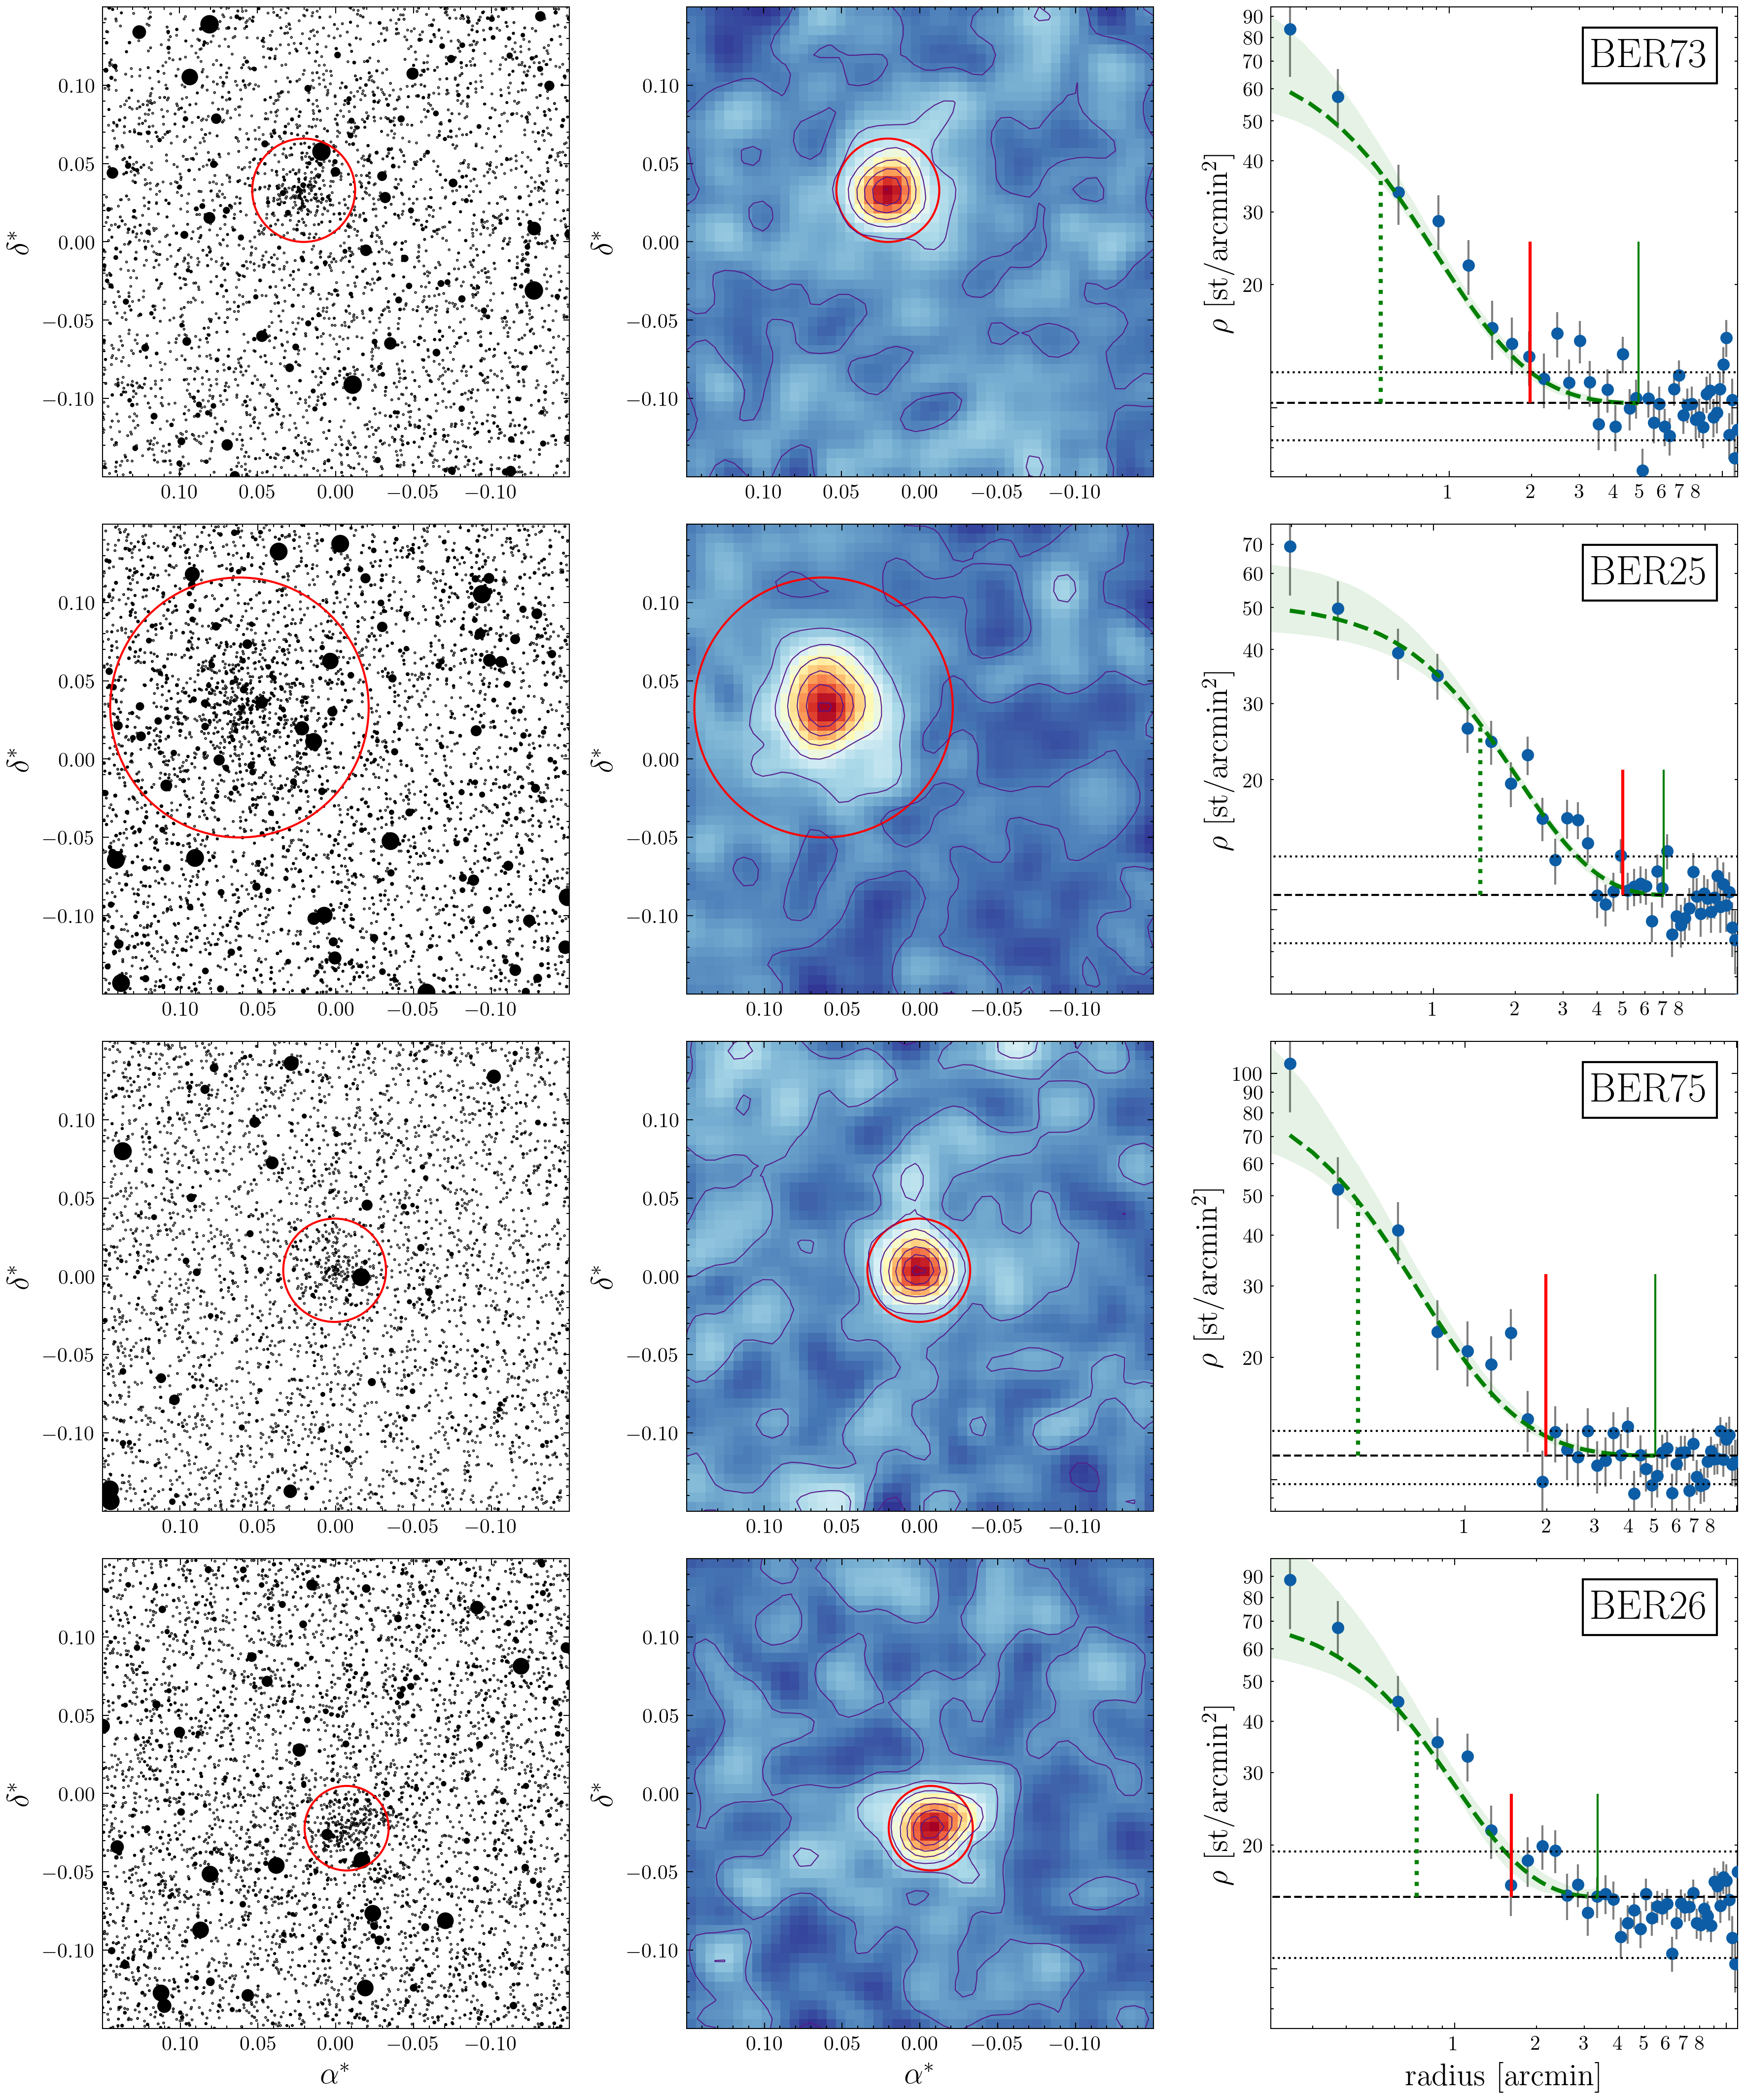
\includegraphics[]{figs/0_struct.png}}
%   \caption{xxx}
%   \label{fig:0struct}
%  \end{figure*}

%  \begin{figure*}
%   \resizebox{\hsize}{!}{\includegraphics[]{figs/4_struct.png}}
%   \caption{xxx}
%   \label{fig:4struct}
%  \end{figure*}

%  \begin{figure*}
%   \resizebox{\hsize}{!}{\includegraphics[]{figs/8_struct.png}}
%   \caption{xxx}
%   \label{fig:4struct}
%  \end{figure*}

%  \begin{figure*}
%   \resizebox{\hsize}{!}{\includegraphics[]{figs/12_struct.png}}
%   \caption{xxx}
%   \label{fig:12struct}
%  \end{figure*}

%  \begin{figure*}
%   \resizebox{\hsize}{!}{\includegraphics[]{figs/16_struct.png}}
%   \caption{xxx}
%   \label{fig:16struct}
%  \end{figure*}

%  \begin{figure*}
%   \resizebox{\hsize}{!}{\includegraphics[]{figs/20_struct.png}}
%   \caption{xxx}
%   \label{fig:20struct}
%  \end{figure*}

% \end{appendix}

\end{document}


